\documentclass[]{tufte-book}

% ams
\usepackage{amssymb,amsmath}

\usepackage{ifxetex,ifluatex}
\usepackage{fixltx2e} % provides \textsubscript
\ifnum 0\ifxetex 1\fi\ifluatex 1\fi=0 % if pdftex
  \usepackage[T1]{fontenc}
  \usepackage[utf8]{inputenc}
\else % if luatex or xelatex
  \makeatletter
  \@ifpackageloaded{fontspec}{}{\usepackage{fontspec}}
  \makeatother
  \defaultfontfeatures{Ligatures=TeX,Scale=MatchLowercase}
  \makeatletter
  \@ifpackageloaded{soul}{
     \renewcommand\allcapsspacing[1]{{\addfontfeature{LetterSpace=15}#1}}
     \renewcommand\smallcapsspacing[1]{{\addfontfeature{LetterSpace=10}#1}}
   }{}
  \makeatother
\fi

% graphix
\usepackage{graphicx}
\setkeys{Gin}{width=\linewidth,totalheight=\textheight,keepaspectratio}

% booktabs
\usepackage{booktabs}

% url
\usepackage{url}

% hyperref
\usepackage{hyperref}

% units.
\usepackage{units}


\setcounter{secnumdepth}{2}

% citations
\usepackage{natbib}
\bibliographystyle{apalike}

% pandoc syntax highlighting

% longtable
\usepackage{longtable,booktabs}

% multiplecol
\usepackage{multicol}

% strikeout
\usepackage[normalem]{ulem}

% morefloats
\usepackage{morefloats}


% tightlist macro required by pandoc >= 1.14
\providecommand{\tightlist}{%
  \setlength{\itemsep}{0pt}\setlength{\parskip}{0pt}}

% title / author / date
\title{LeaRning R in ChemistRy at Reed College}
\author{Chester Ismay}
\date{2016-09-02}

\usepackage{booktabs}
\usepackage{longtable}
\usepackage{framed,color}
\usepackage{float}
\floatplacement{figure}{H}
\usepackage[parfill]{parskip}
\definecolor{shadecolor}{RGB}{248,248,248}

\ifxetex
  \usepackage{letltxmacro}
  \setlength{\XeTeXLinkMargin}{1pt}
  \LetLtxMacro\SavedIncludeGraphics\includegraphics
  \def\includegraphics#1#{% #1 catches optional stuff (star/opt. arg.)
    \IncludeGraphicsAux{#1}%
  }%
  \newcommand*{\IncludeGraphicsAux}[2]{%
    \XeTeXLinkBox{%
      \SavedIncludeGraphics#1{#2}%
    }%
  }%
\fi

%% Need to clean up
\newenvironment{rmdblock}[1]
  {\begin{shaded*}
  \begin{itemize}
  \renewcommand{\labelitemi}{
    \raisebox{-.7\height}[0pt][0pt]{
  %    {\setkeys{Gin}{width=3em,keepaspectratio}\includegraphics{images/#1}}
    }
  }
  \item
  }
  {
  \end{itemize}
  \end{shaded*}
  }
%% Probably can be omitted
\newenvironment{rmdnote}
  {\begin{rmdblock}{note}}
  {\end{rmdblock}}
\newenvironment{rmdcaution}
  {\begin{rmdblock}{caution}}
  {\end{rmdblock}}
\newenvironment{rmdimportant}
  {\begin{rmdblock}{important}}
  {\end{rmdblock}}
\newenvironment{rmdtip}
  {\begin{rmdblock}{tip}}
  {\end{rmdblock}}
\newenvironment{rmdwarning}
  {\begin{rmdblock}{warning}}
  {\end{rmdblock}}
\newenvironment{learncheck}
  {\begin{rmdblock}{warning}}
  {\end{rmdblock}}
\newenvironment{review}
  {\begin{rmdblock}{warning}}
  {\end{rmdblock}}

% To tweak tufte layout
\geometry{
  left=0.8in, % left margin
  textwidth=35pc, % main text block
  marginparsep=1pc, % gutter between main text block and margin notes
  marginparwidth=8pc % width of margin notes
}

\begin{document}

\maketitle



{
\setcounter{tocdepth}{1}
\tableofcontents
}

\chapter{Introduction}\label{intro}

In the HTML version of this book, you can alo download the PDF version
of the book by clicking on PDF button in the top toolbar of the page.
HTML is the preferred format but the PDF format may be preferred for
some readers. Links to the different GIFs directly found in the HTML
version are provided in the PDF version.

This resource is designed to assist students in CHEM 101/102 in using
RStudio and R Markdown to complete their labs. A more general reference
to the specifics of R, RStudio and R Markdown is available in a
different free book \href{http://ismayc.github.io/rbasics-book}{here}.
This resource will show you GIFs explaining how to do some common
procedures you'll need to do to complete labs. In addition, it will
provide more details about the specifics of the different lab templates
available in the \texttt{chemistr} R package. Each chapter of this book
will correspond to each of the different labs.

If further clarification is needed on any other aspect of the book,
please email \href{mailto:cismay@reed.edu}{me} with a reference to the
error/area where more guidance is necessary. More advanced users are
encouraged to create a GitHub issue
\href{https://github.com/ismayc/rbasics/issues}{here}. Pull requests on
GitHub for typos or improvements are also welcome and you can easily do
so by clicking on the Edit button near Search at the top of the HTML
version of the book.

This book will evolve and be updated as needed based on feedback. You
can always check the date below to see when the book was last updated.
It is recommended that you use Google Chrome as your browser since GIFs
sometimes do not load automatically with other browsers.

\textbf{Book was last updated:}

\begin{verbatim}
## [1] "By cismay on Friday, September 02, 2016 17:38:28 PDT"
\end{verbatim}

\chapter{Starting The Labs}\label{begin}

\section{Working in RStudio Server}\label{working-in-rstudio-server}

\subsection{Logging in and initial
screen}\label{logging-in-and-initial-screen}

The RStudio Server provides a web-based way to run analyses in R. This
means that you will only need an internet connection and a web browser
to run your analyses. Your professor or administrator will provide you
with a link to the web location of your RStudio Server. After entering
the link, you'll see a page that looks something like:

\begin{figure}

{\centering 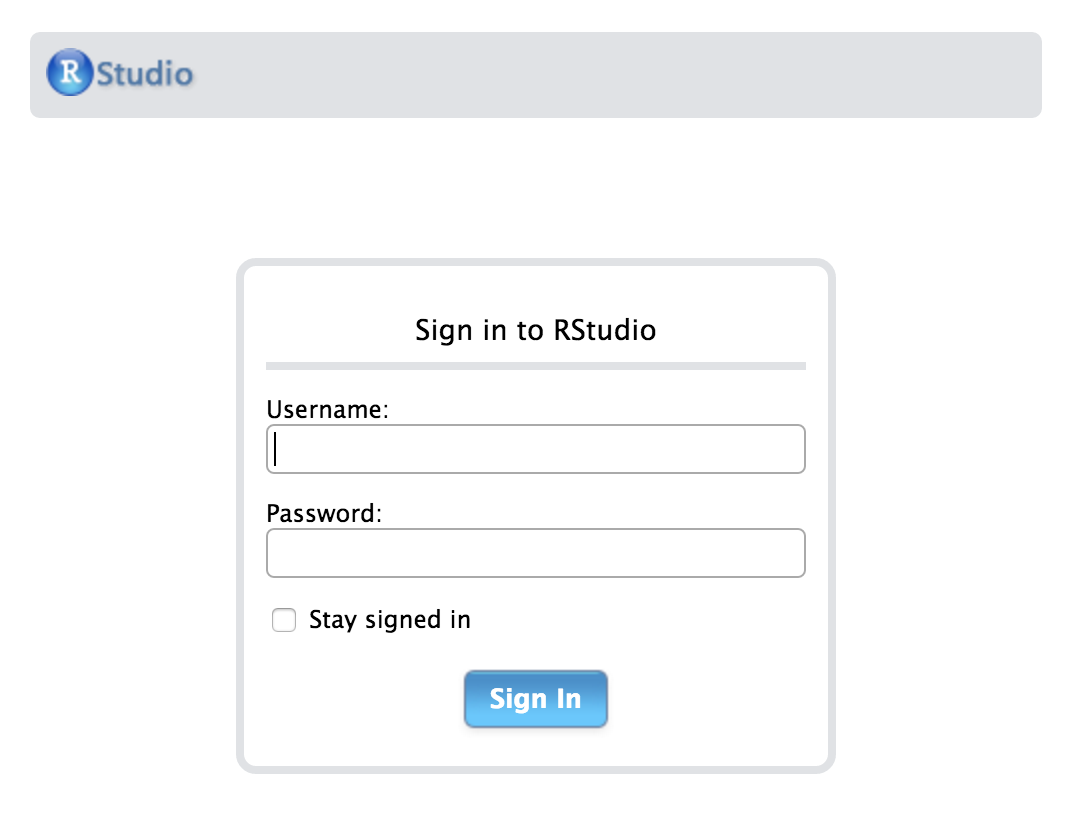
\includegraphics[width=\textwidth]{screenshots/server_login} 

}

\caption[Login page for RStudio Server]{Login page for RStudio Server}\label{fig:serverlogin}
\end{figure}

After logging in with your username and password, you should see a
layout similar to what follows.

\begin{figure}

{\centering 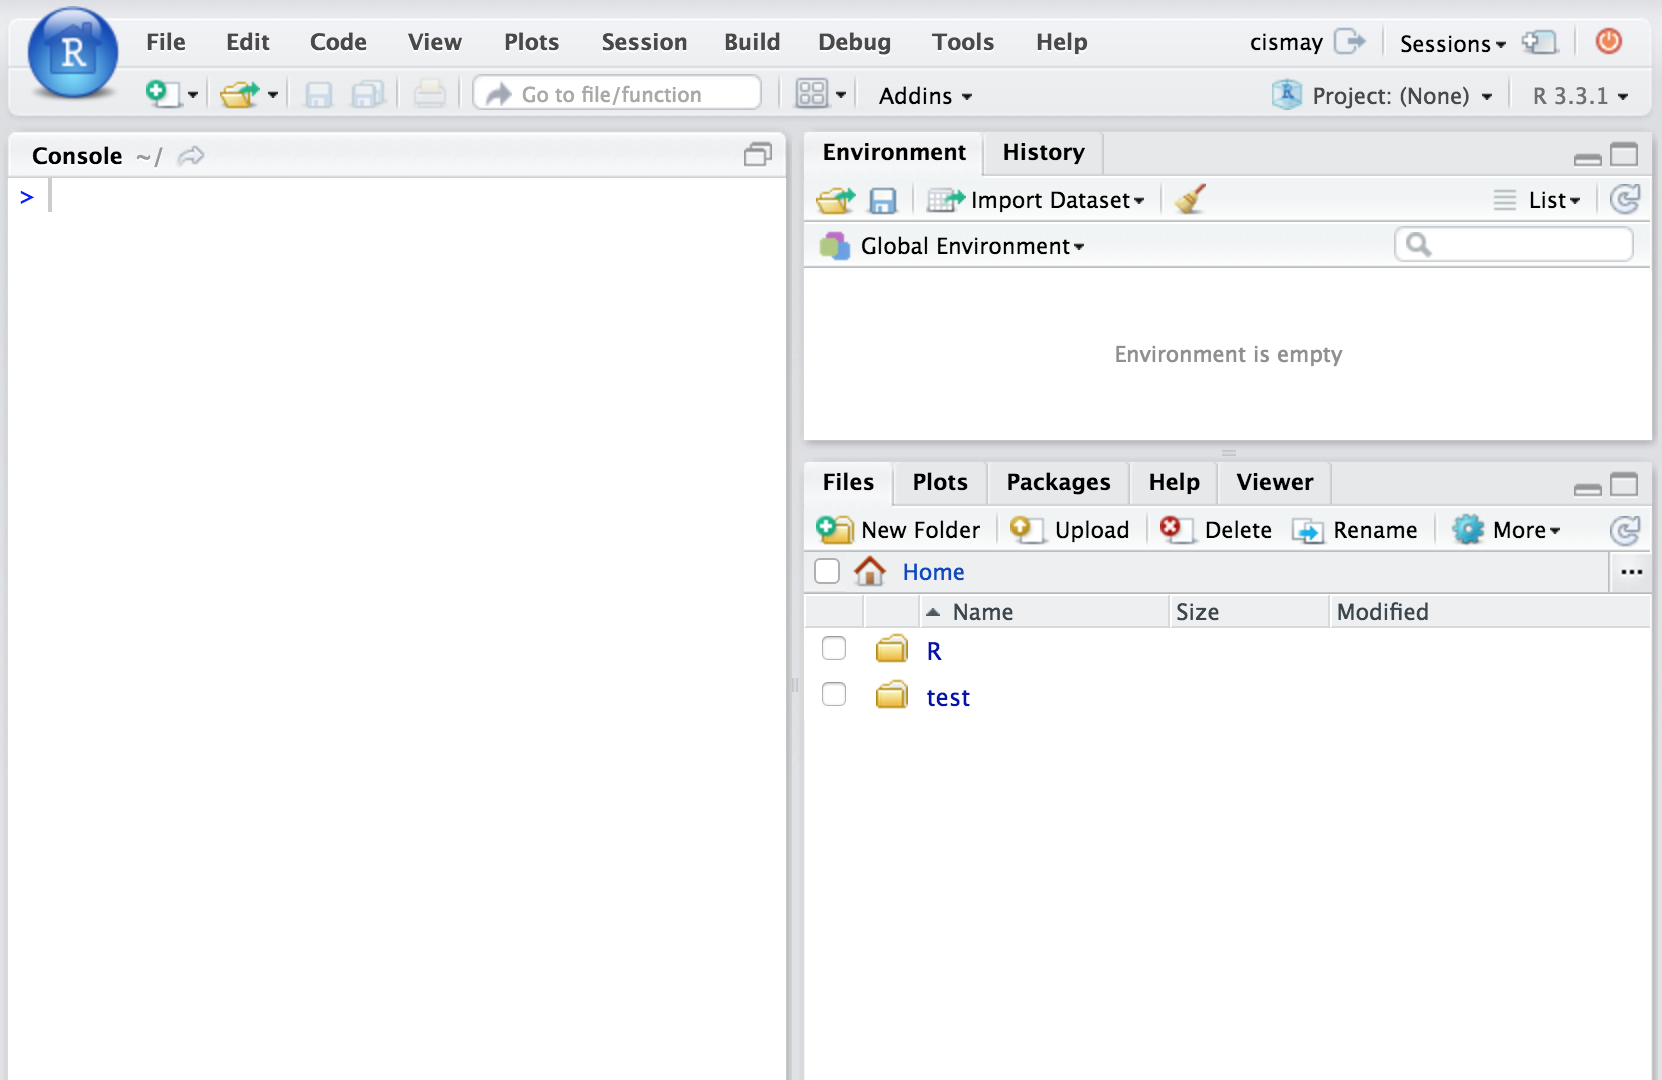
\includegraphics[width=\textwidth]{screenshots/initial_rstudio} 

}

\caption[Initial page for RStudio Server]{Initial page for RStudio Server}\label{fig:initialrstudio}
\end{figure}

\subsection{Basic Workflow with
RStudio}\label{basic-workflow-with-rstudio}

A good habit to get into whenever you start a new project with R code is
to create a new RStudio project to go along with it. RStudio project
files have the extension \texttt{.Rproj} and store metadata that goes
along with the documents you've saved and information about the R
environment you are working in. More information about RStudio projects
is available from RStudio, Inc.
\href{https://support.rstudio.com/hc/en-us/articles/200526207-Using-Projects}{here}.

If you are sharing homework or lab assignments with your instructor
using RStudio Server, for example, it might make sense to create an
RStudio project, share it with your instructor, and then create new
folders for each lab. We will follow this example below.

The GIF below shows you how to create a new RStudio project called
\texttt{initial} and also your first R Markdown file. Note that you also
may see a description about what version of R is running on your initial
login like shown in the GIF below in the Console pane.

\vspace{0.1in}

\begin{center}\footnotesize{\url{https://raw.githubusercontent.com/ismayc/rbasics-book/gh-pages/gifs/proj_rmd.gif}}\end{center}

\vspace{0.1in}

We have our \textbf{first\_rmarkdown.Rmd} file set up.

\subsection{Sharing Projects on RStudio Server
Pro}\label{sharing-projects-on-rstudio-server-pro}

You will now see an example of how to share this project with another
user. This will enable you and collaborators (other students, your
instructor, etc.) to work on the \textbf{Rmd} file at the same time.
This is similar to working on a Google Doc at the same time as someone
else.

RStudio Server comes in a couple different formats and you'll need to
make sure you (or your IT administrator) have installed RStudio Server
Pro to use the Shared Projects feature. You can find more information
from RStudio, Inc. on this
\href{https://support.rstudio.com/hc/en-us/articles/211659737-Sharing-Projects-in-RStudio-Server-Pro}{here}.
Below is an example GIF of sharing this \textbf{initial.Rproj} project
file with another user of the RStudio Server.

\vspace{0.1in}

\begin{center}\footnotesize{\url{https://raw.githubusercontent.com/ismayc/rbasics-book/gh-pages/gifs/share_proj.gif}}\end{center}

\vspace{0.1in}

Both myself and \texttt{bottk} can now work together on this project. We
can type our commentary and code into \textbf{first\_rmarkdown.Rmd} or
other files and save files to the common folder where
\textbf{initial.Rproj} resides.

\vspace*{0.2in}

\noindent\textbf{Help}\vspace*{0.1in}

\bibliography{bib/packages.bib,bib/books.bib,bib/articles.bib}



\end{document}
